% 자동 생성: scripts/plot_composite_final_dist.py — 수정은 스크립트에서
% 데이터: composite-final-20260814T114929Z cases.jsonl (rho, n={'seq2': 493, 'pool': 493})
\documentclass[tikz,border=2pt]{standalone}
\usepackage{pgfplots}
\pgfplotsset{compat=1.18}
\definecolor{seqblue}{HTML}{3A6FE0}
\definecolor{poolred}{HTML}{D5484A}
\begin{document}
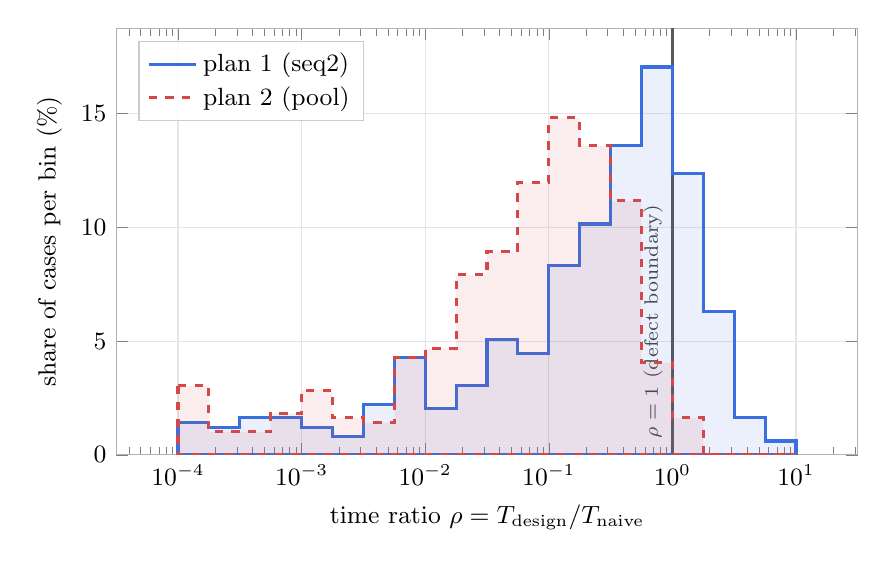
\begin{tikzpicture}
\begin{axis}[
  width=11cm, height=7cm,
  xmode=log,
  xlabel={time ratio $\rho = T_{\mathrm{design}} / T_{\mathrm{naive}}$},
  ylabel={share of cases per bin (\%)},
  ymin=0,
  grid=major, grid style={gray!20},
  axis line style={gray!60},
  tick label style={font=\small},
  label style={font=\small},
  legend style={at={(0.03,0.97)}, anchor=north west, font=\small,
                 draw=gray!40, fill=white, fill opacity=0.9, text opacity=1},
  legend cell align=left,
]
\draw[black!65, line width=0.9pt] (axis cs:1,0) -- (axis cs:1,\pgfkeysvalueof{/pgfplots/ymax});
\node[gray!50!black, font=\scriptsize, anchor=south west, rotate=90]
  at (axis cs:1,0.3) {$\rho=1$ (defect boundary)};
\addplot[seqblue, solid, line width=1.1pt, const plot,
  fill=seqblue, fill opacity=0.10, draw opacity=1] coordinates {
(0.0001,1.420)(0.000177828,1.217)(0.000316228,1.623)(0.000562341,1.623)(0.001,1.217)
(0.00177828,0.811)(0.00316228,2.231)(0.00562341,4.260)(0.01,2.028)(0.0177828,3.043)
(0.0316228,5.071)(0.0562341,4.462)(0.1,8.316)(0.177828,10.142)(0.316228,13.590)
(0.562341,17.039)(1,12.373)(1.77828,6.288)(3.16228,1.623)(5.62341,0.609)
(10,0.609)} \closedcycle;
\addlegendentry{plan 1 (seq2)}
\addplot[poolred, dashed, line width=1.1pt, const plot,
  fill=poolred, fill opacity=0.10, draw opacity=1] coordinates {
(0.0001,3.043)(0.000177828,1.014)(0.000316228,1.014)(0.000562341,1.826)(0.001,2.840)
(0.00177828,1.623)(0.00316228,1.420)(0.00562341,4.260)(0.01,4.665)(0.0177828,7.911)
(0.0316228,8.925)(0.0562341,11.968)(0.1,14.807)(0.177828,13.590)(0.316228,11.156)
(0.562341,4.057)(1,1.623)(1.77828,0.000)(3.16228,0.000)(5.62341,0.000)
(10,0.000)} \closedcycle;
\addlegendentry{plan 2 (pool)}
\end{axis}
\end{tikzpicture}
\end{document}
